% 79-48(79쪽) — 원에 내접하는 사각형 $\pt{ABCD}$(원문 「오른쪽 그림」). 스캔 화질이 낮아 TikZ 로 다시 그림.
% 라벨은 원문 것만: 꼭짓점 A·B·C·D 와 각 $\alpha$·$\beta$. 원문 그림도 어림 그림이라 치수·눈금은 적지 않는다.
% $\tan\alpha+\sin\beta$(답)가 그림에서 읽히지 않게 각의 크기는 원문처럼 실제 값과 다른 어림으로 둔다.
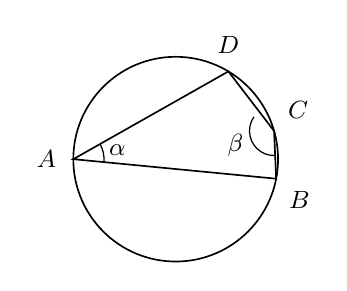
\begin{tikzpicture}[line width=0.6pt, x=1.3cm, y=1.3cm]
  \draw (0,0) circle (1);
  \coordinate (A) at (180:1);
  \coordinate (B) at (-11:1);
  \coordinate (C) at (16:1);
  \coordinate (D) at (59:1);
  \draw (A) -- (B) -- (C) -- (D) -- cycle;
  \draw[line width=0.45pt] (A) ++(-5.5:0.30) arc (-5.5:29.5:0.30);
  \draw[line width=0.45pt] (C) ++(-87.4:0.24) arc (-87.4:-214.9:0.24);
  \node[font=\small] at (-0.57,0.09) {$\alpha$};
  \node[font=\small] at (0.585,0.138) {$\beta$};
  \node[font=\small, anchor=east] at (-1.07,0) {$\pt{A}$};
  \node[font=\small, anchor=north west] at (1.01,-0.22) {$\pt{B}$};
  \node[font=\small, anchor=south west] at (1.00,0.30) {$\pt{C}$};
  \node[font=\small, anchor=south] at (0.515,0.93) {$\pt{D}$};
\end{tikzpicture}
